\section{Introduction}

A supervised machine learning problem is one which a learning algorthim is presented a set of training data and attempts to find an unkown function which maps the training values to the correct answer.
Typically the training set, denoted $S$, is a set of the form $\left \{ (\vec{x}_1,y_1), (\vec{x}_2,y_2), \dots, (\vec{x}_n,y_n) \right \}$ where $\vec{x}_i$ is vector of some features of the problem.
Examples of problem features include discrete or real valued items such as height, weight, age, zip code, grade point average, starting salary, and telephone number (as just a few)  which might make up the features of a person.
The $y_i$ are the class of the training feature $\vec{x}_i$ belongs to; these might be University of Tennessee students or Carnegie Mellon students.
In this examples students with a zip code of 15213 are likely to be Tartans, while students with a zip code of 37916 are like to be Volunteers.
The challenge arises from examples have overlaping features; for example this author as a former Tartan and current Vol would be difficult to classify by zip code.
The learning algorthims job is then to find a hypothesis $h$ that corrrectly classifies a student as a Volunteer of Tartan based on the features providied.
This learning process can then be defined as finding the hypothesis that has the least error (incorrect classifications) on the training data set while extending to examples outside of the training space.

\subsection{Support Vector Machines}
Support Vector Machines (SVM) are a supervised learning technqiue in which hyperplanes are constructed in a high dimensional space to which the features are mactched.
SVMs find the hyperplanes that are the farthest away from all of mapped features in order to provide excellent training performance while still maintaing the ability to generalize to new instances; i.e. SVMs are maximal margin classifiers.
For a binary classification the decision function of the SVM is the dot product of the weight vector and the training example in the feature space added to a bias vector as shown in Equation \ref{eq:BCSVM}.

\begin{equation}
\label{eq:BCSVM}
f \left ( \vec{x} \right ) = \left \langle \vec{w} \phi(\vec{x}) \right \rangle + \vec{b}
\end{equation}
where $\phi(\vec{x})$ is a mapping to the higher dimensional space.
The learning in the SVM is then finding the optimal values of the weight vector $\vec{w}$ and the basis $\vec{b}$.

The radial basis function (Equation \ref{eq:RBF}) is a common kernal function used to map the input vector $\vec{x}$ into a higher dimension.
\begin{equation}
\label{eq:RBF}
k \left ( \vec{x}_i , \vec{x}_j \right ) = exp \left ( - \frac{\left \| \vec{x}_i - \vec{x}_j \right \|}{2\sigma^2} \right ) 
\end{equation}
The maximal margin is ensured by minimizing:
\begin{equation}
\label{eq:Min}
g(\vec{w},\eta) = \frac{1}{2} \left \| \vec{w} \right \| + C \sum_{i=1}^N \zeta_i
\end{equation}
subject to:
\begin{equation}
\label{eq:Constraint}
y_i( \left \langle \vec{w},\phi(\vec{x}) \right \rangle + b ) \ge 1-\zeta_i, ~~~\zeta_i \ge 0
\end{equation}
where $\zeta_i$ is the $i$th slack varaible and C is the regulariazation parameter \cite{li_adaboost_2008}.
Something about how we are trying to elarge the margin

\subsection{Ensamble Classifers}
Given an individiual classifier $h$, an enamble of classifers can be constructed of a set of indvidual classifers, $H={h_1, h_2,\dot, h_n}$.

As long as the individual classifers have uncorrelated errors when any single classifer is incorrect the other classifiers in the ensamble might correctly classify the example.

\subsection{Boosting}
Unbalanced data sets (data sets in which a majority of the values come from one class, see Figure \ref{fig:ClassDist}) are difficult for classification schemes to learn because the minority class is not well represented and tends to be thought as noise for the classifer.
Often classifiers are trained from unblananced data sets by artifically reblaning the dataset by sampling techniques; i.e. up-sampling (sampling more from the minoarty class) and down-sampling (sampling less from the majoirty class).
Boosting is an ensamble learning method in which a set of weights is maintained over the training samples and adaptively adjusted after each training itteration according to the ones that are misclasified \cite{li_adaboost_2008}.
By maintaining a weight distribution over all of the training examples, these weights could be updated to emphasize the training examples that are misclassified incorrectly.  These incorrectly classified examples could then be learned in a refinement of the classifier or by training adding a new classifer to the ensamble with the new weights.
\begin{figure*}[ht!]
	\centering
	\begin{subfigure}[b]{0.3\textwidth}
		\centering
		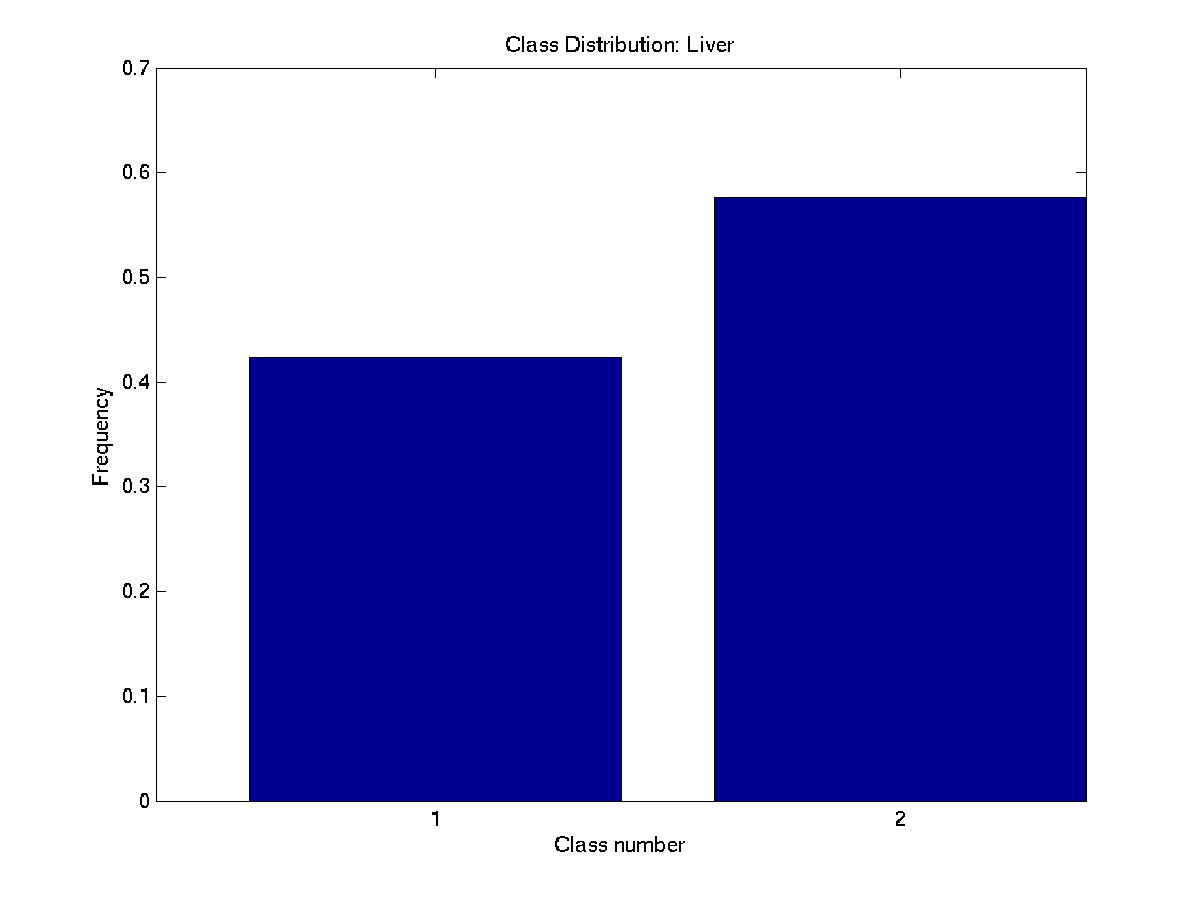
\includegraphics[width=\textwidth]{Liver_ClassDist}
        \caption{Liver}
	\end{subfigure}%
	~
	\begin{subfigure}[b]{0.3\textwidth}
		\centering
		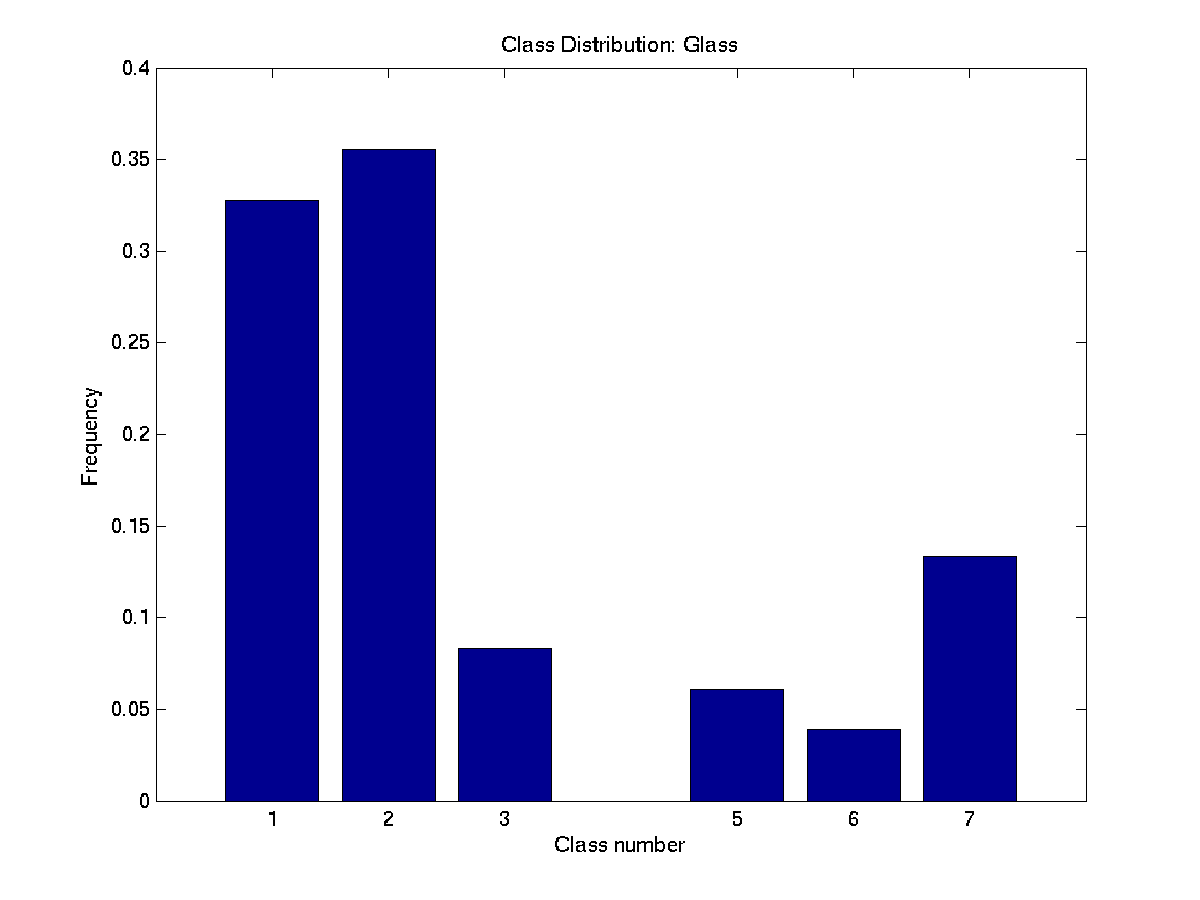
\includegraphics[width=\textwidth]{Glass_ClassDist}
        \caption{Glass}
	\end{subfigure}	
    ~
	\begin{subfigure}[b]{0.3\textwidth}
		\centering
		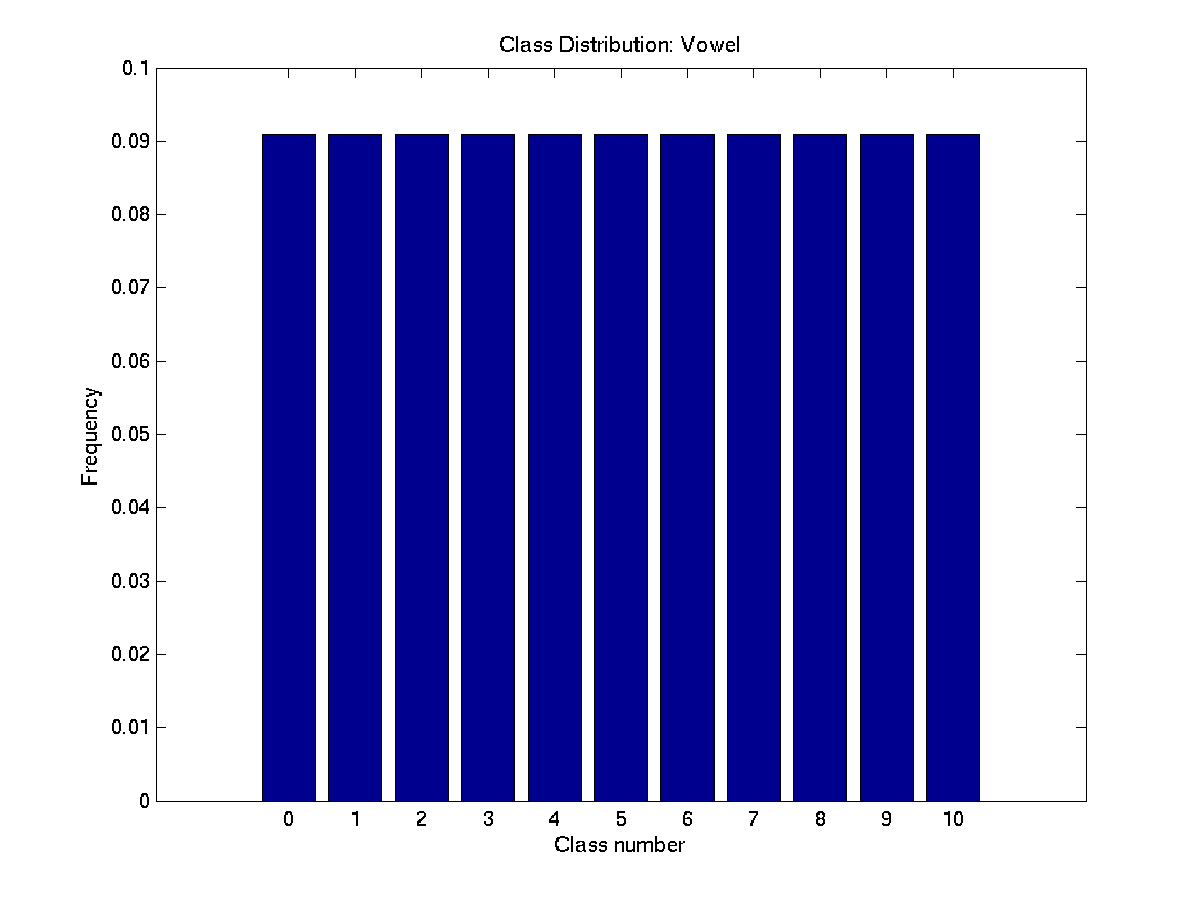
\includegraphics[width=\textwidth]{Vowel_ClassDist}
        \caption{Vowel}
	\end{subfigure}%
	\caption{Distribution of Class Data}
	\label{fig:ClassDist}
\end{figure*}
